\begin{frame}[c]{}

\centering
\huge
Lecture 2:\\
Design Spaces in Machine Learning
\end{frame}
%----------------------------------------------------------------------
%----------------------------------------------------------------------
\begin{frame}[c]{Where are we? The big picture}

\begin{itemize}
	\item Introduction
	\item[$\to$] Background
	\begin{itemize}
		\item[$\to$] Design spaces in ML
		\item Experimentation and visualization
	\end{itemize}
	\item Hyperparameter optimization (HPO)
	\begin{itemize}
	  \item Bayesian optimization
	  \item Other black-box techniques
	\end{itemize}
	\item Speeding up HPO with multi-fidelity optimization
	\item Pentecost (Holiday) -- no lecture
	\item Architecture search I + II
	\item Meta-Learning
	\item Learning to learn $\&$ optimize
	\item Beyond AutoML: algorithm configuration and control
	\item Project announcement and closing
\end{itemize}


\end{frame}
%----------------------------------------------------------------------
%----------------------------------------------------------------------
\begin{frame}[c]{Learning Goals}

After this lecture, you will be able to \ldots

\begin{itemize}
  \item identifiy design decisions of machine learning algorithms
  \item explain different types of design decisions and there relations
  \item create design spaces
  \item discuss the pro and cons of different design space approaches
\end{itemize}

\end{frame}
%----------------------------------------------------------------------
%----------------------------------------------------------------------
\begin{frame}[c]{Simples Design Decisions: Selection of Algorithm}

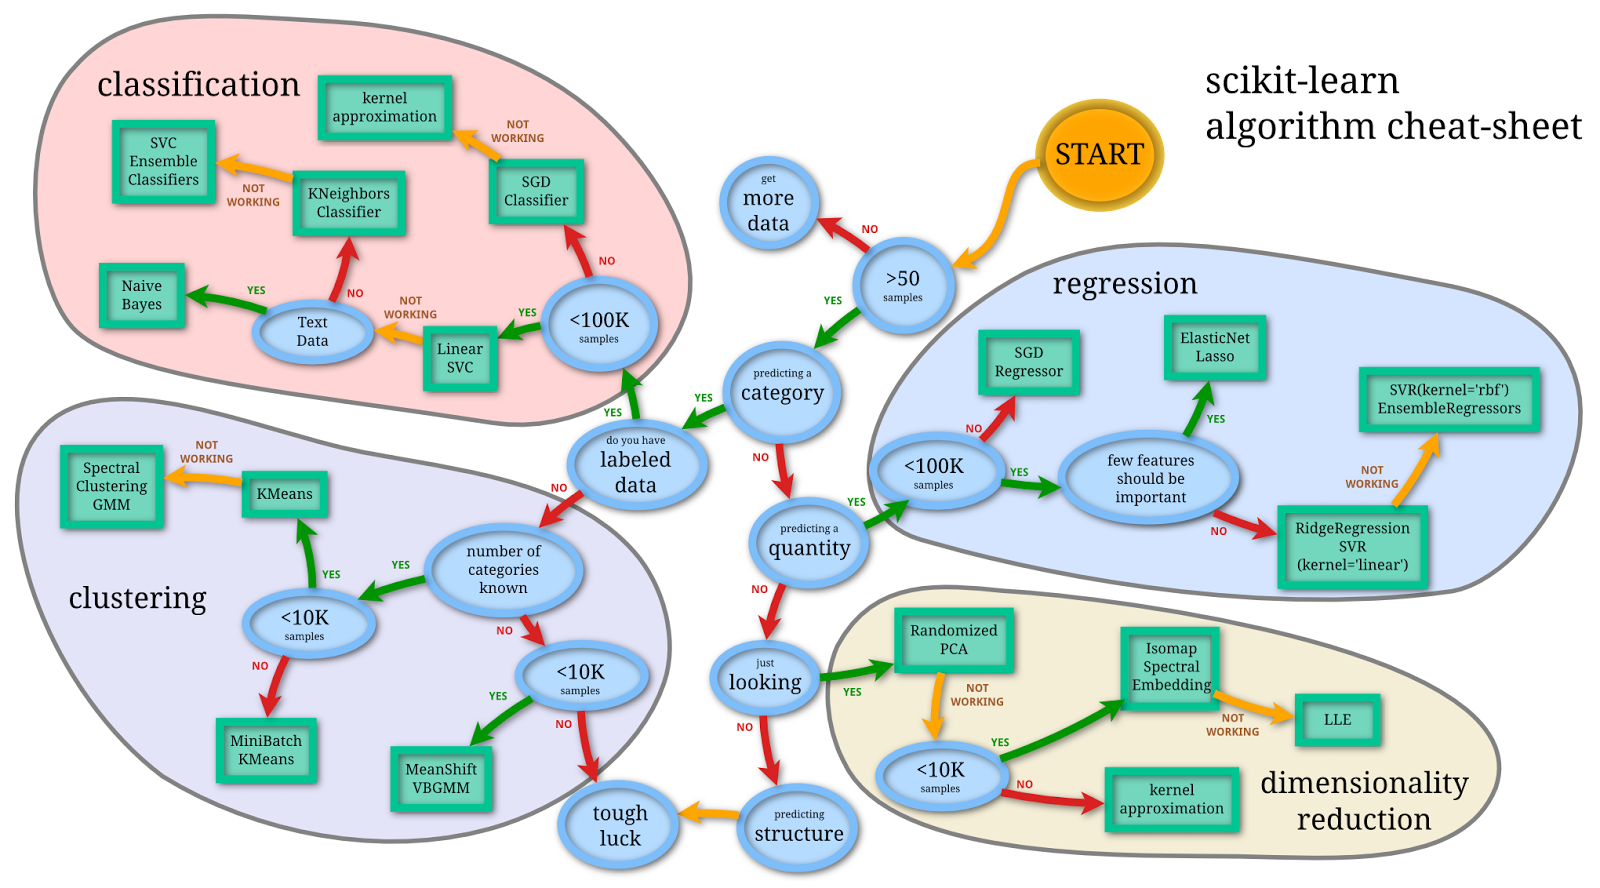
\includegraphics[width=1.0\textwidth]{images/sklearn-cheat}


\end{frame}
%----------------------------------------------------------------------
%----------------------------------------------------------------------
\begin{frame}[c]{Simples Design Decisions: Selection of Algorithm}

\begin{itemize}
  \item categorical design decison: $\{ \algo_1, \algo_2, \algo_3, \ldots, \algo_n\}$
  \begin{itemize}
	\item random forest (RF), support vector machine (SVM),\\ gradient boosting (GB), \ldots
    \item there is no ordering between algorithms
    \item set notation
  \end{itemize}
  \pause
  \item if we would run all of them and each takes (on average) $t$ seconds:\\
  $t \cdot n$ seconds
  \pause
  \smallskip
  \item in addition, choose pre-processing algorithm: $\{\algo_1^P, \algo_2^P, \algo_3^P, \ldots \algo_l^P \}$
  \begin{itemize}
    \item PCA, feature selection, random kitchen sinks, \ldots
  \end{itemize}
  \item if we only use one preprocessor and one ML algorithm, brute force would need:\\
  $t \cdot n \cdot l$
\end{itemize}

\end{frame}
%----------------------------------------------------------------------
%----------------------------------------------------------------------
\begin{frame}[c]{Design Space of Support Vector Machines}

\centering
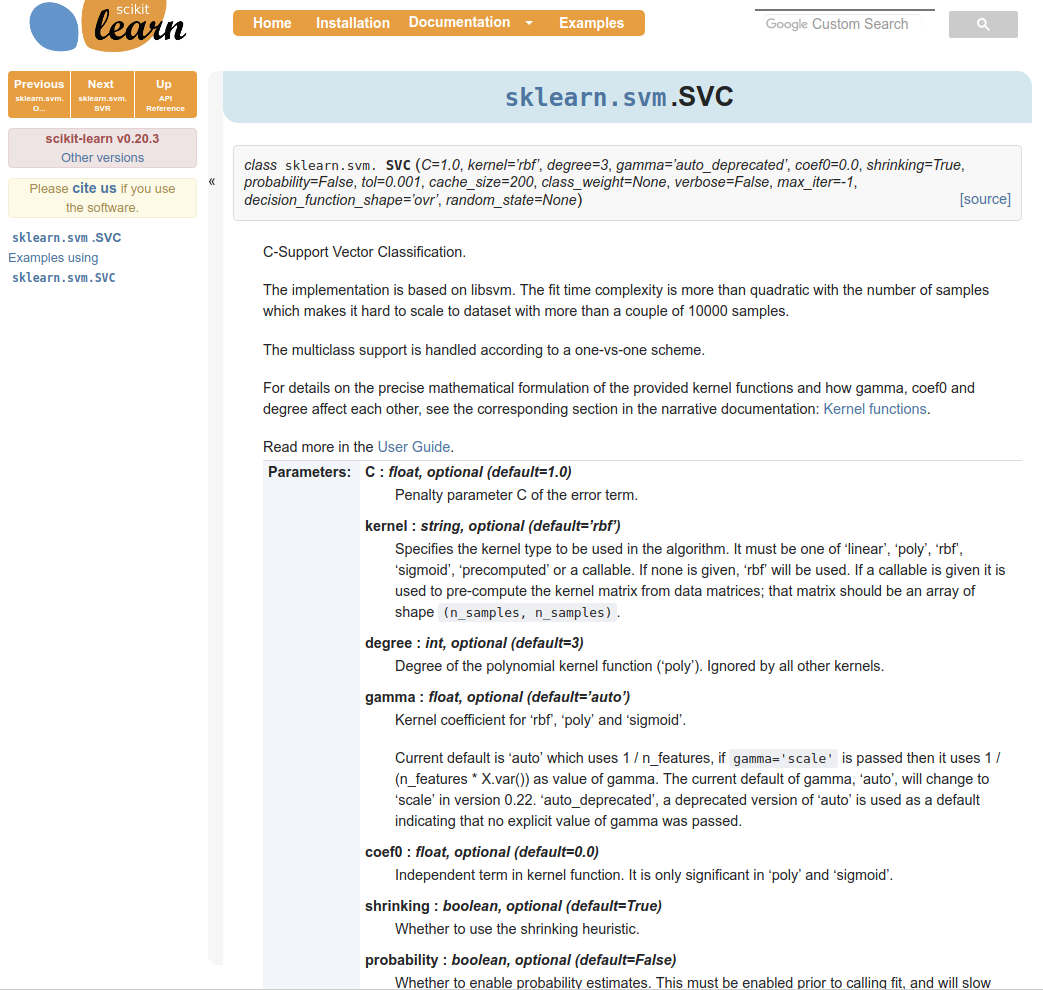
\includegraphics[width=0.7\textwidth]{images/sklearn_svm_doc.png}

\end{frame}
%----------------------------------------------------------------------
%----------------------------------------------------------------------
\begin{frame}[c]{Design Space of Support Vector Machines}

\begin{block}{Hyperparameter Optimization (HPO; informal)}
Given
\begin{itemize}
  \item a dataset
  \item a set of hyperparameters of a machine learning algorithms
  \item a cost metric (e.g., predictive error)
\end{itemize}
we want to find the hyperparameter settings minimizing the cost metric wrt the dataset. 
\end{block}

\begin{block}{Hyperparameter Types of SVM}
\begin{description}
  \item[C] float hyperparameter
  \item[Kernel] categorical hyperparameter
  \item[Degree] integer hyperparamerter
  \item[gamma] float hyperparamerter
  \item \ldots
\end{description}
\end{block}

\end{frame}
%----------------------------------------------------------------------
%----------------------------------------------------------------------
\begin{frame}[c]{Hyperparameter Types}

\begin{description}
	\item[categorical] set of values (not sorted, no distance)
	\begin{itemize}
	  \item \texttt{kernel \{linear, rbf, poly, sigmoid\}}
	\end{itemize}
	\pause
	\item[ordinal] list of values with uniform distance
	\begin{itemize}
	  \item no example in SVM design space
	  \item \texttt{size [small, medium, large]}
	\end{itemize}
	\pause
	\item[integer] bounded range of integers
	\begin{itemize}
	  \item \texttt{degree [1, 5]}
	\end{itemize}
	\pause
	\item[float] bounded range of floats
	\begin{itemize}
	  \item \texttt{gamma\_value [0.0001, 8.0]}
	\end{itemize}
\end{description}

\end{frame}
%----------------------------------------------------------------------
%----------------------------------------------------------------------
\begin{frame}[c,fragile]{Design Space}

The combination of several hyperparameter ranges $\pcs_i$ creates a design space:
$\pcs = \theta_1 \times \theta_2 \times \theta_3 \ldots \times \theta_n$ 

\pause
\bigskip

For example the design space of a SVM, would include:

\begin{verbatim}
kernel categorical {linear, rbf, poly, sigmoid}
degree integer [1, 5]
gamma_value float [0.0001, 8.0]
\end{verbatim}

\end{frame}
%----------------------------------------------------------------------
%----------------------------------------------------------------------
\begin{frame}[c]{Concept of Defaults}

\begin{itemize}
  \item We assume that each algorithm has a default
  \begin{itemize}
    \item often a robust setting of the algorithm if you don't want to change it
    \item default often provided by developer, e.g.,\\
   		  in its documentation or the paper
  \end{itemize}
  \item We use the default to start our search for hyperparameter optimization
  \begin{itemize}
    \item if we know a reasonable configuration,\\ we should start with a random configuration?
    \item Goal: find something which is better than the default
    \item Pro: Can help us to start in good region of the design space
    \item Contra: We might start being trapped in local optimum.
  \end{itemize}
\end{itemize}

Example: the default \texttt{kernel} is the RBF-kernel\\
\texttt{kernel categorical \{linear, rbf, poly, sigmoid\}[rbf]}

\end{frame}
%----------------------------------------------------------------------
%----------------------------------------------------------------------
\begin{frame}[c]{Slide}


\end{frame}
%----------------------------------------------------------------------
%----------------------------------------------------------------------
\begin{frame}[c]{Slide}


\end{frame}
%----------------------------------------------------------------------
%----------------------------------------------------------------------
\begin{frame}[c]{Slide}


\end{frame}
%----------------------------------------------------------------------
%----------------------------------------------------------------------
\begin{frame}[c]{Slide}


\end{frame}
%----------------------------------------------------------------------
%----------------------------------------------------------------------
\begin{frame}[c]{Slide}


\end{frame}
%----------------------------------------------------------------------
%----------------------------------------------------------------------
\begin{frame}[c]{Slide}


\end{frame}
%----------------------------------------------------------------------
%----------------------------------------------------------------------
\begin{frame}[c]{Slide}


\end{frame}
%----------------------------------------------------------------------
%----------------------------------------------------------------------
\begin{frame}[c]{Slide}


\end{frame}
%----------------------------------------------------------------------
%----------------------------------------------------------------------
\begin{frame}[c]{Slide}


\end{frame}
%----------------------------------------------------------------------
%----------------------------------------------------------------------
\begin{frame}[c]{Slide}


\end{frame}
%----------------------------------------------------------------------
%----------------------------------------------------------------------
\begin{frame}[c]{Slide}


\end{frame}
%----------------------------------------------------------------------
%----------------------------------------------------------------------
\begin{frame}[c]{Slide}


\end{frame}
%----------------------------------------------------------------------
%----------------------------------------------------------------------
\begin{frame}[c]{Slide}


\end{frame}
%----------------------------------------------------------------------
%----------------------------------------------------------------------
\begin{frame}[c]{Slide}


\end{frame}
%----------------------------------------------------------------------
%----------------------------------------------------------------------
\begin{frame}[c]{Slide}


\end{frame}
%----------------------------------------------------------------------
%----------------------------------------------------------------------
\begin{frame}[c]{Slide}


\end{frame}
%----------------------------------------------------------------------



%----------------------------------------------------------------------
\begin{frame}[c]{Learning Goals}

Now, you should be able to \ldots

\begin{itemize}
  \item identifiy design decisions of machine learning algorithms
  \item explain different types of design decisions and there relations
  \item create design spaces
  \item discuss the pro and cons of different design space approaches
\end{itemize}

\end{frame}
%----------------------------------------------------------------------

